\documentclass[11pt]{article}
\usepackage{lineno}
\usepackage{graphicx}

\begin{document}

\begin{titlepage}

\newcommand{\HRule}{\rule{\linewidth}{0.5mm}} 

\center % Center everything on the page
 
%----------------------------------------------------------------------------------------
%	HEADING SECTIONS
%----------------------------------------------------------------------------------------

\textsc{\LARGE Texas A$\&$M University}\\[1.5cm] 
\textsc{\Large Summer Research Paper 1}\\[0.5cm] % 

%----------------------------------------------------------------------------------------
%	TITLE SECTION
%----------------------------------------------------------------------------------------

\HRule \\[0.4cm]
{ \huge \bfseries Exploring the Euclidean Algorithm}\\[0.4cm] 
\HRule \\[1.5cm]
 
%----------------------------------------------------------------------------------------
%	AUTHOR SECTION
%----------------------------------------------------------------------------------------

\begin{minipage}{0.4\textwidth}
\begin{flushleft} \large
\emph{Authors:}\\
Stephen \textsc{Capps}\\
Sarah \textsc{Sahibzada}\\
Taylor \textsc{Wilson}
\end{flushleft}
\end{minipage}
~
\begin{minipage}{0.4\textwidth}
\begin{flushright} \large
\emph{Supervisor:} \\
Dr. Sarah \textsc{Pollock} 
\end{flushright}
\end{minipage}\\[4cm]

%----------------------------------------------------------------------------------------
%	DATE SECTION
%----------------------------------------------------------------------------------------

{\large \today}\\[3cm] 

%----------------------------------------------------------------------------------------
%	LOGO SECTION
%----------------------------------------------------------------------------------------

%\includegraphics{Logo}\\[1cm] 
 
%----------------------------------------------------------------------------------------

\vfill 

\end{titlepage}

\tableofcontents
\newpage
\newpage

\section{Iterations' Distribution}
	\subsection{Brief Introduction} $ $ \indent This section investigates the number of iterations it takes to complete the Euclidean Algorithm. For example, the number of iterations it take to complete gcd$(42,36)$ is $2$, as shown below.
		$$\mathrm{gcd}(42,36) = 6:$$
	\begin{equation}
		42 = 1 * 36 + 6
	\end{equation}
	\begin{equation}
		36 = 6 * 6 + 0
	\end{equation}
Some other examples are as follows:

$$\mathrm{gcd}(78,45) = 3 \quad| \quad\mathrm{Iterations}: 5$$
$$\mathrm{gcd}(689,456) = 1 \quad|\quad \mathrm{Iterations}: 6$$
$$\mathrm{gcd}(8394,238) = 2 \quad|\quad \mathrm{Iteration}: 7$$
		
This leads us to an investigation into what numbers yield the longest iterations, and the distribution of these iterations.

	\subsection{Results} $ $
	\indent The results were quiet surprising, as most distributions were almost perfectly Gaussian. The following figures are different distributions of different iterations of various gcd combinations.\\
	
	\begin{figure}
		\centering
		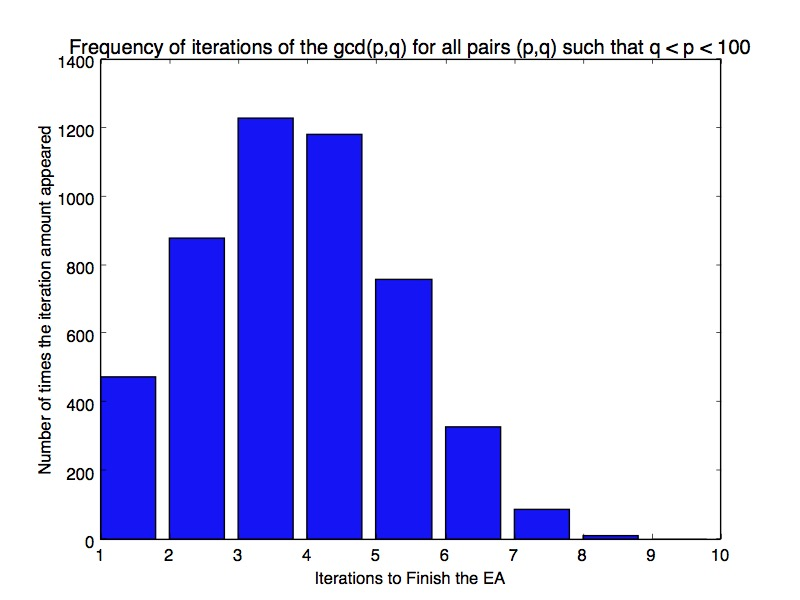
\includegraphics[scale=.45]{2digit_iterationfreq.jpg}
		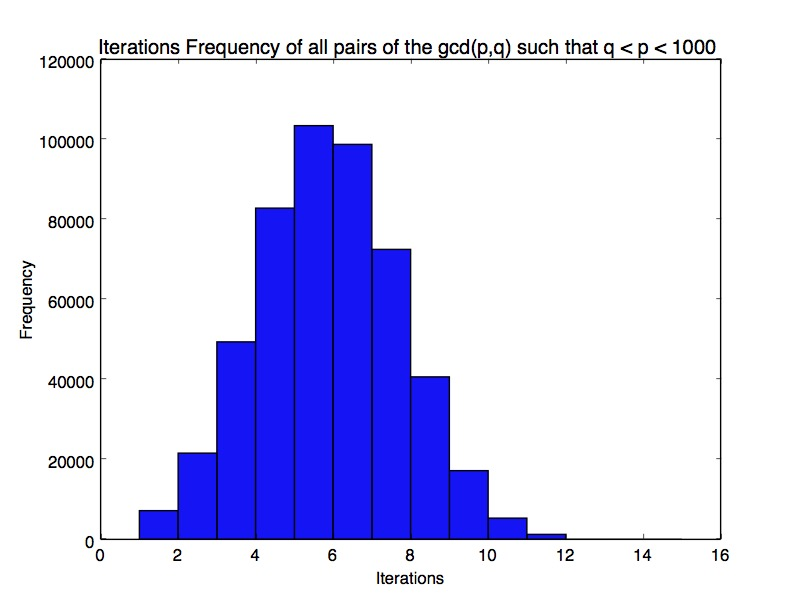
\includegraphics[scale=.45]{3digit_iteration_freq.jpg}\\
	\end{figure}
	
	\begin{figure}
		\centering
		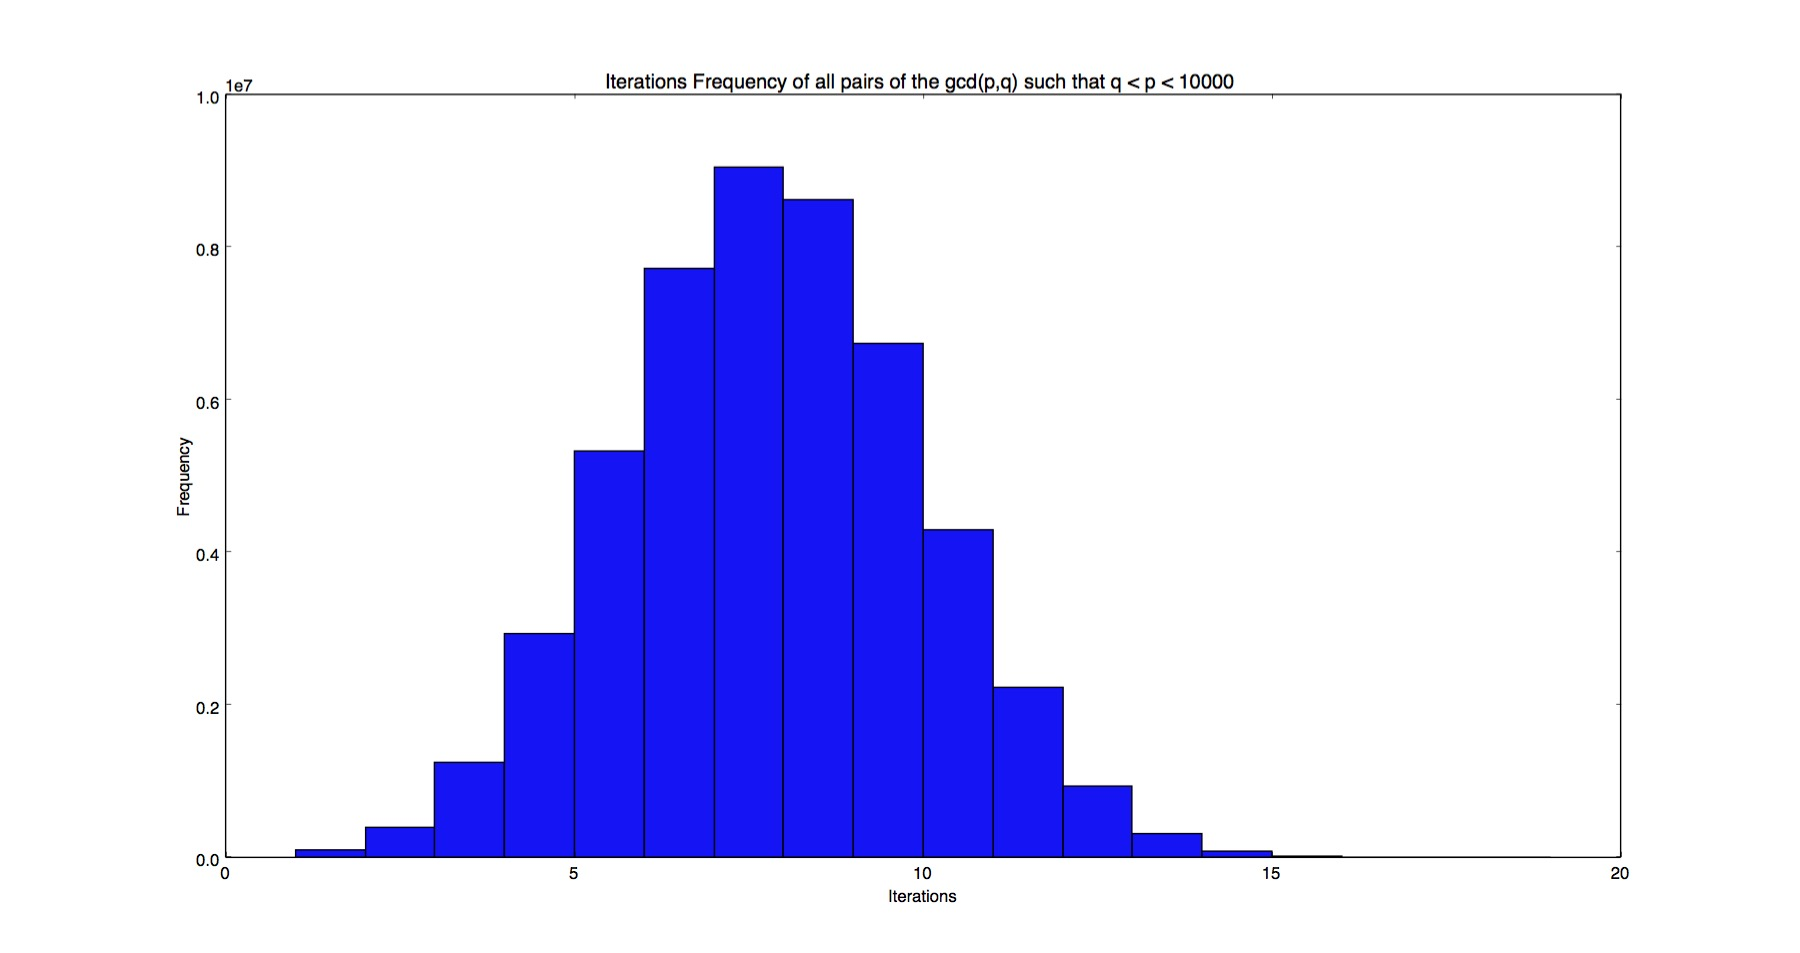
\includegraphics[scale=.3]{4digit_iteration_freq.jpg}
		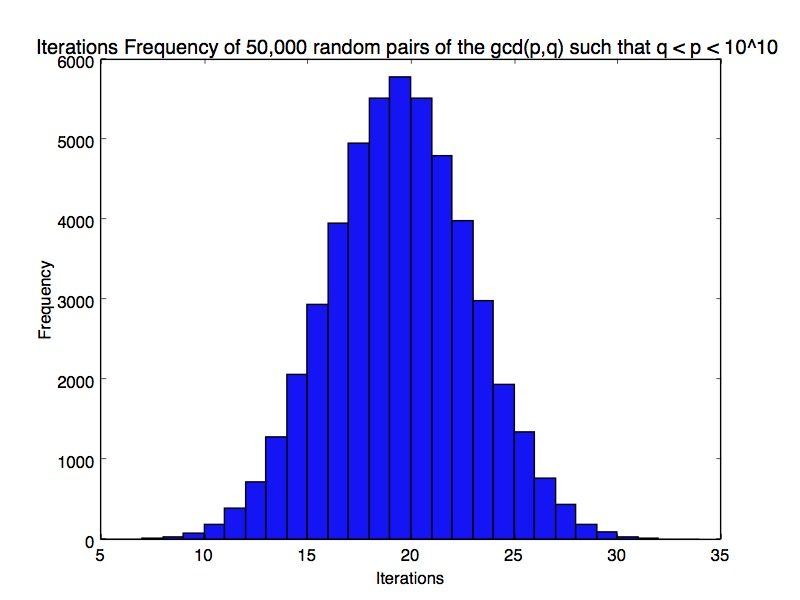
\includegraphics[scale=.45]{10_digit_numbers.jpg}
		
	\end{figure}
	
	\begin{figure}
		\centering
		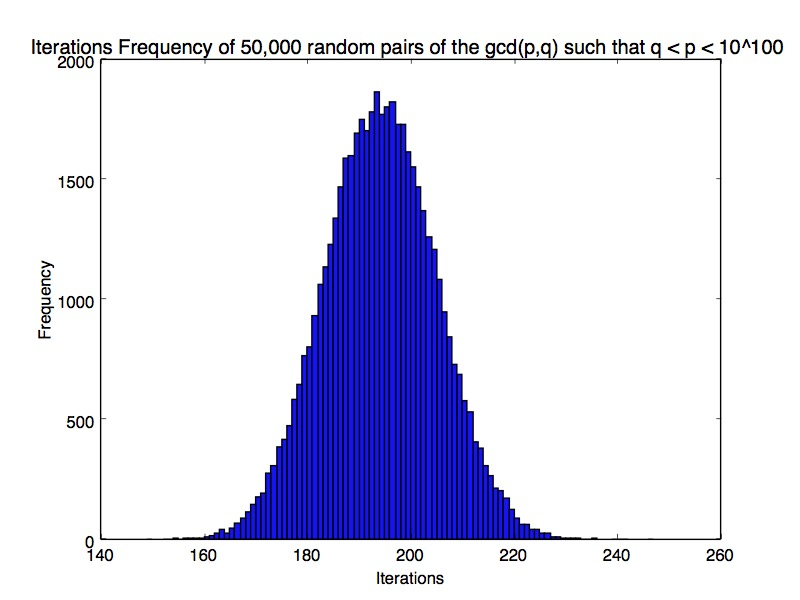
\includegraphics[scale=.45]{100_digit_numbers_freq.jpg}
		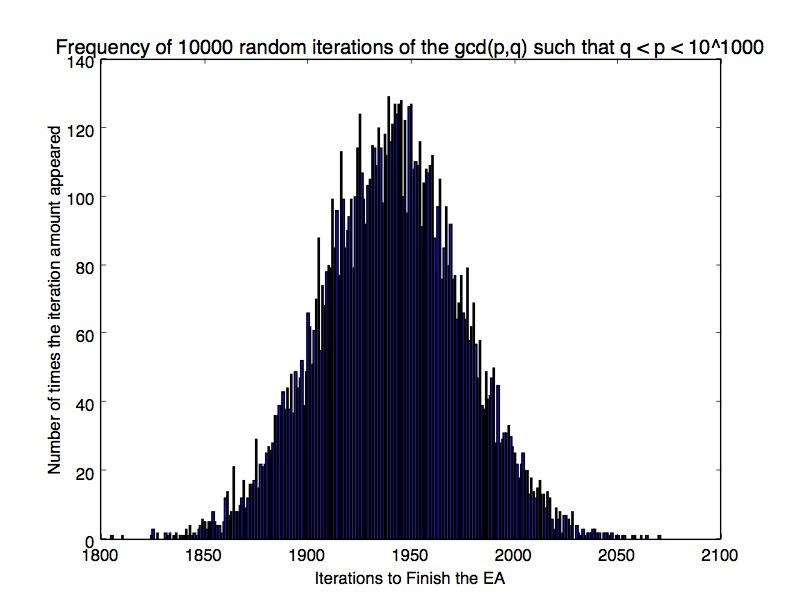
\includegraphics[scale=.45]{1000_digit_numbers.jpg}
		
	\end{figure}
	\newpage
	As the number of digits we consider increases, the distribution	 becomes continuously more Gaussian. However, after a point our computational resources restrict us from checking all pairs p,q with some large upper bound. Thus, we restrict ourselves by picking a set amount of pairs and calculating their distribution. You can see this progression as the figures continue.\\
	
	Note the increasing mean iterations as we climb the upper bound.
	
	\subsection{Conclusion}
\newpage
	
\section{[Section 2 title]}
	\subsection{[if needed]}
	\subsection{[if needed]}
	\subsection{[if needed]}

\newpage

\section{[Section 3 title]}
	\subsection{[if needed]}
	\subsection{[if needed]}
	\subsection{[if needed]}




\end{document}